\documentclass[12pt,letterpaper]{article}
\usepackage{graphicx,textcomp}
\usepackage{natbib}
\usepackage{setspace}
\usepackage{fullpage}
\usepackage{color}
\usepackage[reqno]{amsmath}
\usepackage{amsthm}
\usepackage{fancyvrb}
\usepackage{amssymb,enumerate}
\usepackage[all]{xy}
\usepackage{endnotes}
\usepackage{lscape}
\newtheorem{com}{Comment}
\usepackage{float}
\usepackage{hyperref}
\newtheorem{lem} {Lemma}
\newtheorem{prop}{Proposition}
\newtheorem{thm}{Theorem}
\newtheorem{defn}{Definition}
\newtheorem{cor}{Corollary}
\newtheorem{obs}{Observation}
\usepackage[compact]{titlesec}
\usepackage{dcolumn}
\usepackage{tikz}
\usetikzlibrary{arrows}
\usepackage{multirow}
\usepackage{xcolor}
\newcolumntype{.}{D{.}{.}{-1}}
\newcolumntype{d}[1]{D{.}{.}{#1}}
\definecolor{light-gray}{gray}{0.65}
\usepackage{url}
\usepackage{listings}
\usepackage{color}
\UseRawInputEncoding

\definecolor{codegreen}{rgb}{0,0.6,0}
\definecolor{codegray}{rgb}{0.5,0.5,0.5}
\definecolor{codepurple}{rgb}{0.58,0,0.82}
\definecolor{backcolour}{rgb}{0.95,0.95,0.92}

\lstdefinestyle{mystyle}{
	backgroundcolor=\color{backcolour},   
	commentstyle=\color{codegreen},
	keywordstyle=\color{magenta},
	numberstyle=\tiny\color{codegray},
	stringstyle=\color{codepurple},
	basicstyle=\footnotesize,
	breakatwhitespace=false,         
	breaklines=true,                 
	captionpos=b,                    
	keepspaces=true,                 
	numbers=left,                    
	numbersep=5pt,                  
	showspaces=false,                
	showstringspaces=false,
	showtabs=false,                  
	tabsize=2
}
\lstset{style=mystyle}
\newcommand{\Sref}[1]{Section~\ref{#1}}
\newtheorem{hyp}{Hypothesis}

\title{Replication Project - Applied Statistical Analysis II}
\date{Due: March 31, 2026}
\author{Matilda Tomatis}

\begin{document}
	
	\maketitle
	\tableofcontents
	\newpage
	
	\section{Introduction}
	
\vspace{0.5cm}
	
\noindent This paper replicates and extends Giani, M., Hope, D., \& Skorge, \O. S. (2022)\footnote{Household education gaps and gender role attitudes. \textit{Political Science Research and Methods}, 10(4), 823--830. doi:10.1017/psrm.2021.16}. The original authors investigate how the educational gap between respondents and their partners affects attitudes towards gender roles; which is operationalised as the difference in approval between a mother and a father holding a full-time job while having a child under the age of three, with the gender of the parent presented as an experimentally varied vignette. More specifically, the study draws on the 2018 European Social Survey, finding that as the educational gap increases in favour of the woman, female respondents tend to hold more egalitarian attitudes. The opposite pattern is observed for their male counterparts. The pattern observed is coherent with a \emph{resource-bargaining} approach. 

\vspace{0.5cm}
\noindent The authors employ a kernel-based interflex model, which allows the coefficient $\beta$ to vary continuously across values of the moderating variable (in this case, the educational gap), rather than imposing a single linear interaction effect. This flexibility comes, however, at the cost of interpretive simplicity. In my contribution, I show that a linear interflex model yields comparable substantive results while remaining considerably easier to interpret and communicate. This matters because replication studies serve not only to verify original findings, but also to assess whether those findings are robust to alternative (and potentially more transparent) modelling choices.

\vspace{0.5cm}
\noindent All the figures reported in this paper are the results of the author's own replication work. 


\vspace{1.5cm}
	
\section{Original Data}

\vspace{0.5cm}

\noindent In their original study, Giani, Hope \& Skorge (2022) build on the centrality of gender attitudes in shaping political and economic choices. They identify two major theoretical frameworks in the literature: \emph{resource-bargaining}, which understands gender attitudes as a function of the relative power of individuals within the household, and \emph{gender identity} theory, which instead understands attitudes as a function of the cost of deviating from stereotypical gender roles.

\noindent The data come from the 2018 European Social Survey (Round 9), a large-scale cross-national survey administered biennially across European countries via face-to-face interviews, covering 19 countries in total.\footnote{Austria, Belgium, Bulgaria, Cyprus, Czechia, Estonia, Finland, France, Germany, Hungary, Ireland, Italy, The Netherlands, Norway, Poland, Serbia, Slovenia, Switzerland, and the United Kingdom.}

\vspace{0.5cm}
\lstinputlisting[language=R, firstline=33, lastline=33]{Replication_Proj_MT.R}

\vspace{0.5cm}


\noindent The dependent variable is a survey question measuring the extent to which respondents approve of a \emph{person} holding a full-time job while having a child under the age of three. Crucially, the survey randomises whether the person referred to is a man or a woman, effectively operationalising gender bias as the difference in approval between a mother and a father in otherwise identical circumstances.

\vspace{0.5cm}
\lstinputlisting[language=R, firstline=143, lastline=145]{Replication_Proj_MT.R}

\vspace{0.5cm}

\noindent The main independent variables are the \emph{educational attainment of the respondent} and of \emph{their partner} (as such, the sample is restricted to respondents who are currently partnered) and the randomised \emph{gender of the parent in the vignette}. The educational gap is computed by taked the respondent's level of education on a 1 to 7 ES-ISCED scale, and subtracting that of the partner from it. The resulting variable, \emph{edu\_diff} ranges on a scale from -6 to 6.

\noindent To assess whether the respondent's own gender moderates the relationship between educational gap and attitudes, the sample is later split into two subsets: one for female respondents and one for male respondents.

\vspace{0.5cm}
\lstinputlisting[language=R, firstline=81, lastline=88]{Replication_Proj_MT.R}

\vspace{0.5cm}

\noindent In addition to the main independent variables, a comprehensive set of controls is included, among them the respondent's income, squared income and the share of females in their family unit. A more substantial viewing of the code relative to the data wrangling can carried out through the \emph{my\_data} R-script. 

\noindent Figure~\ref{fig:visualisation_1a} reports that the distribution of male and female respondents does not differ systematically across the proposed gender in the vignette.
\vspace{0.5cm}

\begin{figure}[H]\centering
	\caption{}
	\label{fig:visualisation_1a}
	\hspace*{-0.65cm}
	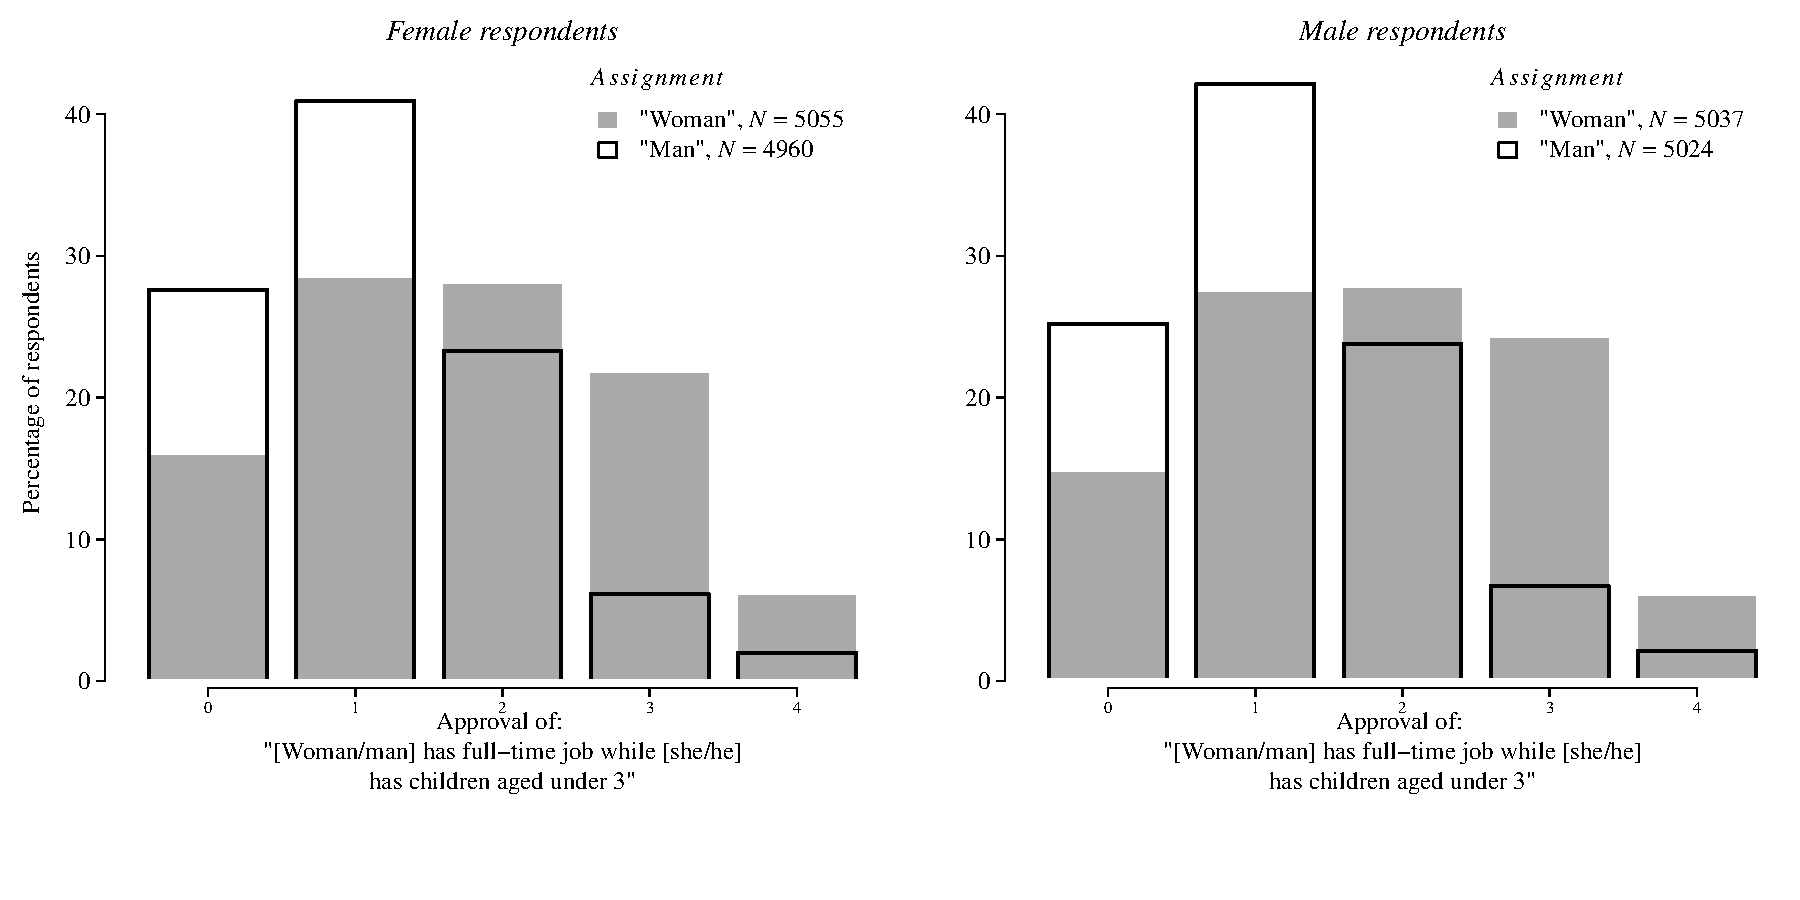
\includegraphics[width=1.1\textwidth]{Figure1a.pdf}
\end{figure}

\noindent Finally, Figure~\ref{fig:visualisation_1b} showcases a balance check confirming that the gender of the respondnet is orthogonal to the distribution of the educational gap (as expected under randomisation).

\begin{figure}[H]\centering
	\caption{}
	\label{fig:visualisation_1b}
	\hspace*{-0.65cm}
	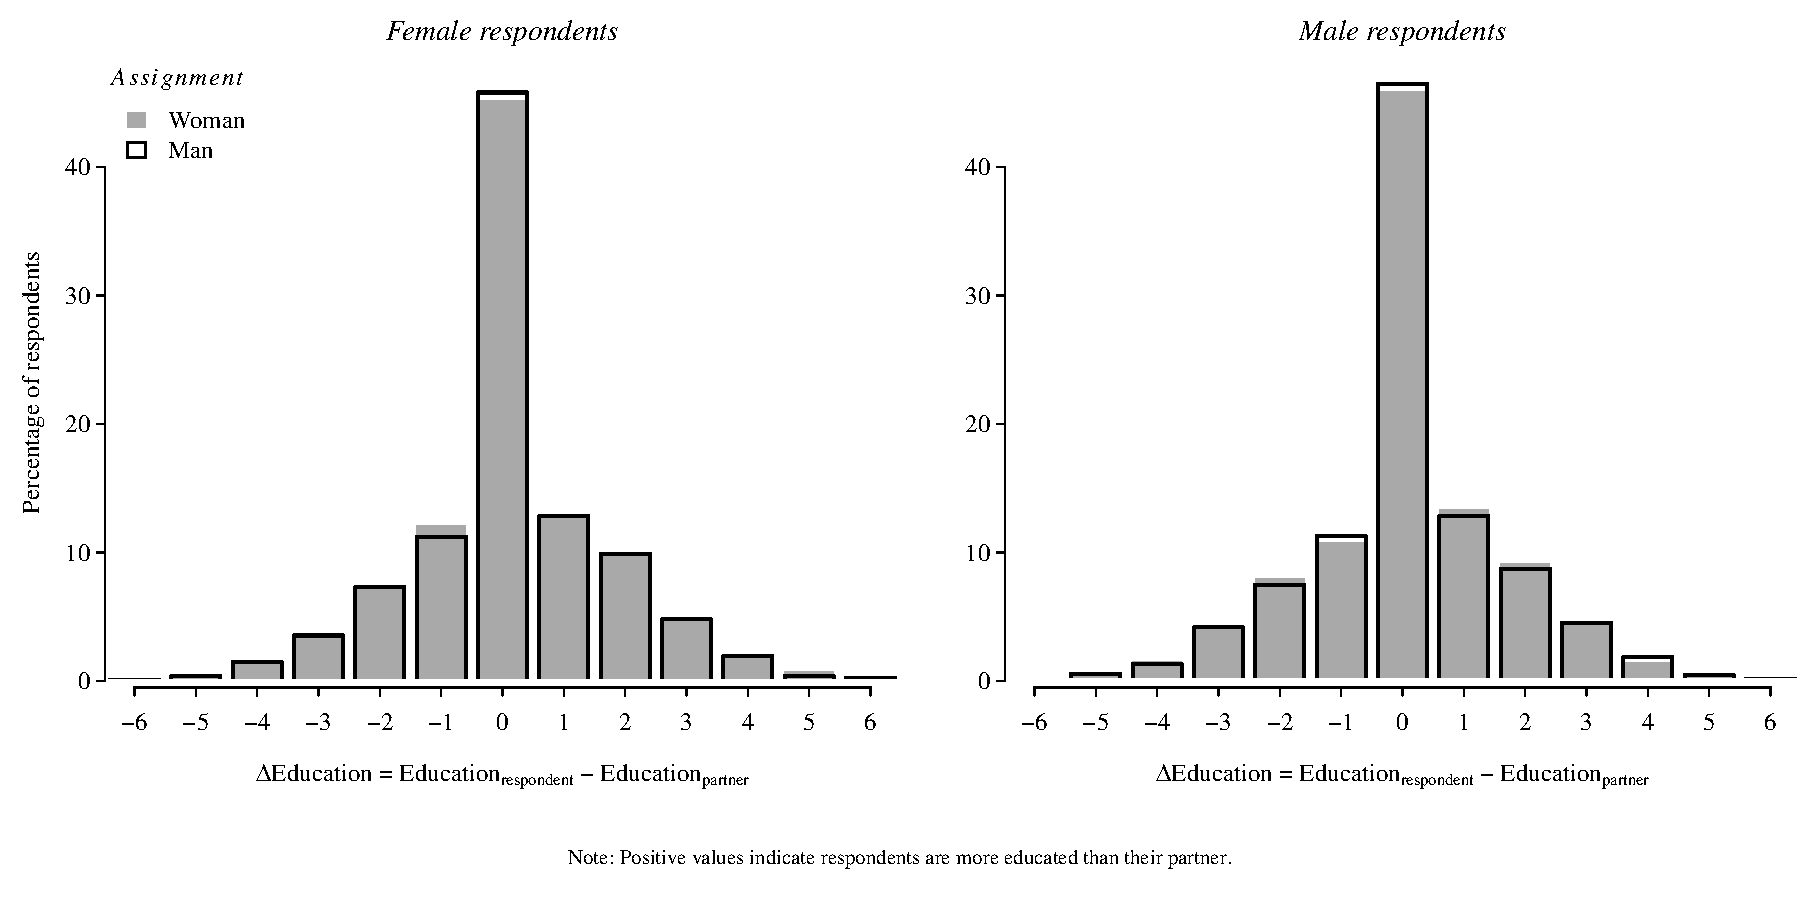
\includegraphics[width=1.1\textwidth]{Figure1b.pdf}
\end{figure}

\vspace{1.5cm}

\section{Original Method \& Findings}

\vspace{0.5cm}

\noindent The authors employ a Gaussian kernel interflex model: a semi-parametric 
model which allows the gender childcare bias to vary non-monotonically across 
levels of the educational gap. Crucially, this flexibility comes at the cost of 
interpretive simplicity, as the model does not yield a single coefficient but 
rather a smooth function estimated at each value of the moderator.

\noindent The formula is defined specifically by the moderating role of educational 
differences. In particular, the element the authors focus on is the marginal gender childcare bias conditional on the household educational gap $\Delta E_{i,c}$, which is captured by the smooth function $g(\cdot)$:

\begin{equation}
	Y_{i,c} = \alpha + f(\Delta E_{i,c}) + g(\Delta E_{i,c}) \cdot B_{i,c} 
	+ \gamma(\Delta E_{i,c}) \cdot Z_{i,c} + \mu_c + \varepsilon_{i,c}
	\label{eq:kernel}
\end{equation}

\noindent where $Y_{i,c}$ is the approval outcome, $B_{i,c}$ is the vignette gender and $Z_{i,c}$ is the vector of controls. Among the controls, notably \textit{education} of the respont is added, as to make sure the model is picking up on the effect of $\Delta E_{i,c}$ net of the person's educational achivement. Moreover, the model controls for country fixed effects ($\mu_c$) and it's estimate through a 500 repetitions bootstrap method. 

\vspace{0.5cm}
\lstinputlisting[language=R, firstline=461, lastline=463]{Replication_Proj_MT.R}

\vspace{0.5cm}
\noindent As previously mentioned, to estimate the gender childcare bias separately for women and men, the original dataset is split into two subsets based on the gender of the respondent.

\vspace{0.5cm}
\lstinputlisting[language=R, firstline=449, lastline=453]{Replication_Proj_MT.R}
\vspace{0.5cm}

\noindent The model is then fit for both subsets. Here a snippet of the code is reported; the model was estimated with identical specifications for female and male respondents.

\vspace{0.5cm}
\lstinputlisting[language=R, firstline=477, lastline=493]{Replication_Proj_MT.R}
\vspace{0.5cm}

\noindent The results of the estimation are reported in Figure~\ref{fig:visualisation_2}. The graphs report the marginal change in gender childcare bias given the respondent and their partner's educational gap, for both men and women.
\noindent Here a snippet of the code to obtain the results is reported.

\vspace{0.5cm}
\lstinputlisting[language=R, firstline=579, lastline=640]{Replication_Proj_MT.R}

\vspace{0.5cm}
\begin{figure}[H]\centering
	\caption{}
	\label{fig:visualisation_2}
	\hspace*{-0.9cm}
	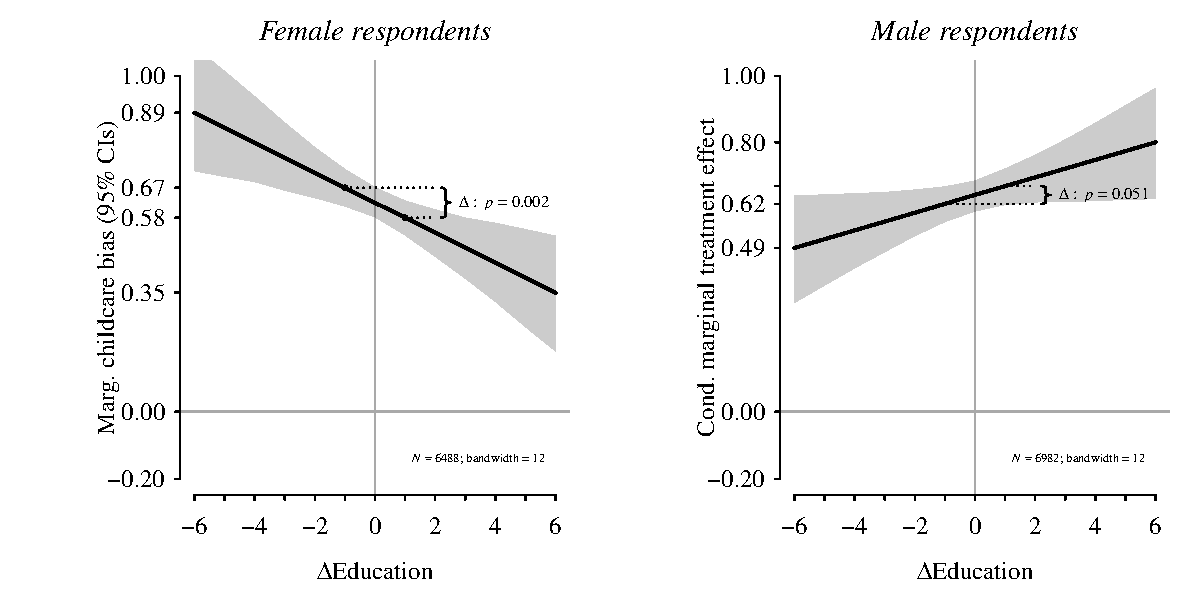
\includegraphics[width=1.1\textwidth]{Figure2.pdf}
\end{figure}

\vspace{0.5cm}
\noindent The results suggest that as the educational gap widens in favour of the respondent, women tend to diminish their gender childcare bias, while their male counterparts tend to show the opposite pattern. The effect appears steeper for female respondents: the reported difference in bias moving from $-1$ to $1$ in $\Delta E_{i,c}$ is $-0.089$, with a statistically significant p-value; on the other hand, the effect for men is $0.053$, with a p-value of $0.051$.

\noindent These results are in line with the \emph{resource-bargaining} framework introduced above. As the respondent holds greater relative power within the household, measured here as a higher level of education, their attitudes tend to reflect those power dynamics. A woman with higher education than her partner shows less bias against mothers holding full-time jobs; conversely, a man in the same position tends to show greater bias.

\noindent The model is also estimated accounting for both the ESS design weight and the post-stratification weight. The results are completely consistent for women and stronly similar for men, as reported in Figure~\ref{fig:visualisation_A2}.

\vspace{0.5cm}
\begin{figure}[H]\centering
	\caption{}
	\label{fig:visualisation_A2}
	\hspace*{-0.9cm}
	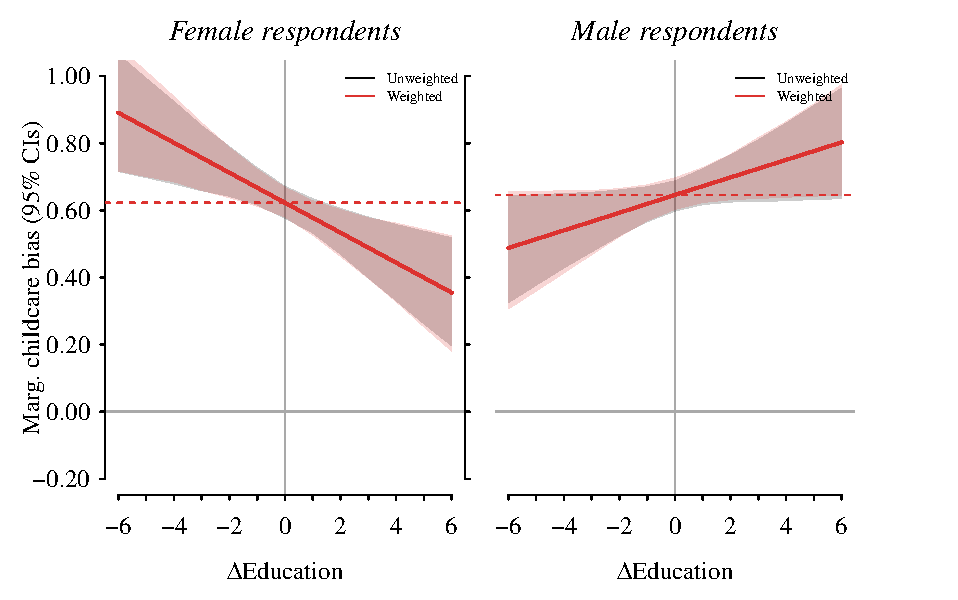
\includegraphics[width=1.1\textwidth]{FigureA2.pdf}
\end{figure}

\vspace{0.5cm}
\noindent Moreover, Figure~\ref{fig:visualisation_A2} helps visualise how the marginal gender childcare bias at $\Delta E_{i,c} = 0$ is notably similar for female and male respondents, suggesting that it is the educational gap itself, rather than baseline attitudes, that drives the divergence between the two groups.

\vspace{1.5cm}

\section{My Contribution}

\vspace{0.5cm}
\noindent Observing the original results (and the replication graphs reported above), I was interested in verifying whether the original authors' choice to employ a Gaussian kernel interflex model was necessary. Such a method is computationally intensive and requires considerable time to run, especially given the original tuning of 10,000 bootstraps. Moreover, it is not particularly intuitive, and the results are not straightforward to interpret and generalise, with the smooth function $g(\cdot)$ being the central inferential target.

\noindent In addition, the results showcase a monotonic decrease for female respondents and a monotonic increase for male respondents, suggesting that a less computationally intensive and more easily interpretable linear model could serve the same purpose. I therefore fit a linear interflex model, retaining the same covariates as well as country fixed effects.

\noindent In such a model, the gender childcare bias is still moderated by the variable \emph{edu\_diff}, however this time $\beta_3$ is the key quantity of interest: a single linear coefficient which captures how the household educational gap reinforces or attenuates the gender childcare bias. Formally:

\begin{equation}
	Y_{i,c} = \alpha + \beta_1 B_{i,c} + \beta_2 \Delta E_{i,c} + 
	\beta_3 (B_{i,c} \times \Delta E_{i,c}) + \gamma Z_{i,c} + 
	\mu_c + \varepsilon_{i,c}
	\label{eq:linear}
\end{equation}

\noindent where $\mu_c$ denotes country fixed effects and all other terms are as defined in Equation~\ref{eq:kernel}. Unlike the kernel model, $\beta_3$ yields a single, interpretable estimate of how the effect of vignette gender on approval changes with the educational gap.

\noindent The coding for the visualisation is an adjustment of the one reported above for Figure~\ref{fig:visualisation_2}; for further detail the full code is reported in the \emph{my\_contribution} R-script. The code reported here refers to the estimation for female respondents; the specification for male respondents is identical but uses the \texttt{dt.m} dataset instead.

\vspace{0.5cm}
\lstinputlisting[language=R, firstline=843, lastline=855]{Replication_Proj_MT.R}
\vspace{0.5cm}

\begin{figure}[H]\centering
	\caption{}
	\label{fig:visualisation_3}
	\hspace*{-0.9cm}
	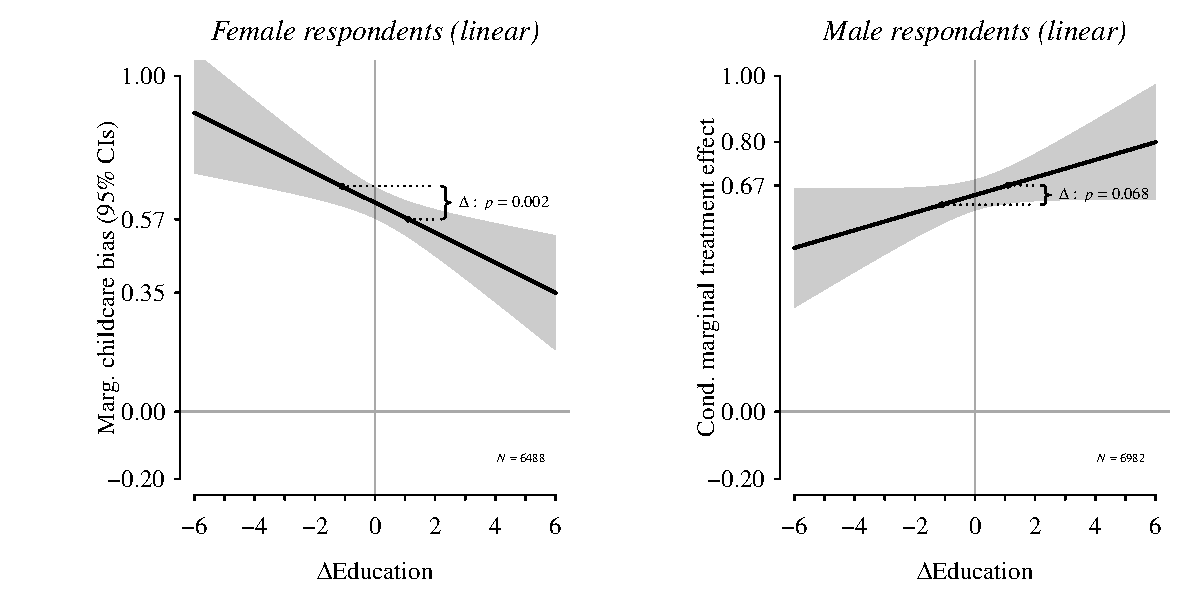
\includegraphics[width=1.1\textwidth]{Figure3_linear.pdf}
\end{figure}
\vspace{0.5cm}

\noindent From a visual inspection, one can observe how the linear and the kernel model deliver similar, if not identical, results. Upon closer numerical inspection, for female respondents the estimated change in the marginal effect and its p-value moving from $\Delta E_{i,c} = -1$ to $1$ are virtually identical across the two specifications, suggesting that the linear model is sufficient.

\begin{verbatim}
	> ix.kern.z.w$diff.estimate
						diff.estimate    sd  z-value  p-value  lower CI(95%)  upper CI(95%)
	1 vs -1        -0.089 0.028  -3.143   0.002        -0.143        -0.035
	> ix.z.w.lin$diff.estimate
						diff.estimate    sd  z-value  p-value  lower CI(95%)  upper CI(95%)
	1 vs -1        -0.089 0.029  -3.106   0.002        -0.146        -0.033
\end{verbatim}

\noindent For male respondents the estimated change is marginally different ($0.053$ vs $0.052$), though the two estimates are noticeably close and both fall short of significance at the 5\% level. Notably, the confidence interval widths are comparable across both specifications, suggesting no meaningful loss of precision under the linear model.

\begin{verbatim}
	> ix.kern.z.m$diff.estimate
						diff.estimate    sd  z-value  p-value  lower CI(95%)  upper CI(95%)
	1 vs -1         0.053 0.027   1.950   0.051         0.001         0.104
	> ix.z.m.lin$diff.estimate
						diff.estimate    sd  z-value  p-value  lower CI(95%)  upper CI(95%)
	1 vs -1         0.052 0.029   1.828   0.068        -0.004         0.109
\end{verbatim}

\noindent The results of the linear model are reported in 
Table~\ref{Tab:Linear_Interflex}. The $\beta_2$ coefficient captures the effect of switching the vignette gender from male to female, at a household educational gap of zero. We find that this raises the disapproval of the parent having a full-time job by approximately 0.623 points for female respondents and 0.646 for male respondents, both statistically significant at the 1\% level.

\noindent The $\beta_3$ coefficient, the focus of our analysis, captures how the household educational gap moderates this gender childcare bias: that is, by how much the effect of the educational gap on approval changes when the vignette gender is female rather than male. We find that, for women, a one-point increase in the educational gap reduces the gender bias by approximately 0.045 points ($p < 0.01$), suggesting that women with higher relative education hold more egalitarian attitudes. For men, the same increase raises the gender bias by 0.026 points ($p < 0.1$), consistent with the opposite pattern. 

\begin{table}[H] \centering 
	\caption{Linear Interflex Models - Core Explanatory Variables} 
	\label{} 
	\begin{tabular}{@{\extracolsep{5pt}}lcc} 
		\\[-1.8ex]\hline 
		\hline \\[-1.8ex] 
		& \multicolumn{2}{c}{\textit{Dependent variable:}} \\ 
		\cline{2-3} 
		\\[-1.8ex] & \multicolumn{2}{c}{Approval} \\ 
		& Women (Linear) & Men (Linear) \\ 
		\\[-1.8ex] & (1) & (2)\\ 
		\hline \\[-1.8ex] 
		Educational Gap ($\beta_1$) & 0.035$^{***}$ & 0.013 \\ 
		& (0.011) & (0.011) \\ 
		& & \\ 
		Vignette Gender ($\beta_2$) & 0.623$^{***}$ & 0.646$^{***}$ \\ 
		& (0.024) & (0.023) \\ 
		& & \\ 
		Edu. Gap $\times$ Vignette Gender ($\beta_3$) & $-$0.045$^{***}$ & 0.026$^{*}$ \\ 
		& (0.015) & (0.014) \\ 
		& & \\ 
		\hline \\[-1.8ex] 
		Observations & 6,488 & 6,982 \\ 
		R$^{2}$ & 0.258 & 0.245 \\ 
		Adjusted R$^{2}$ & 0.254 & 0.241 \\ 
		Residual Std. Error & 0.943 (df = 6450) & 0.961 (df = 6944) \\ 
		\hline 
		\hline \\[-1.8ex] 
		\textit{Note:}  & \multicolumn{2}{r}{$^{*}$p$<$0.1; $^{**}$p$<$0.05; $^{***}$p$<$0.01} \\ 
	\end{tabular} 
	\label{Tab:Linear_Interflex}
\end{table} 

\vspace{1.5cm}

\section{Conclusion}

\vspace{0.5cm}

\noindent My contribution corroborates the substantial findings of Giani, Hope \& Skorge (2022), obtaining the same robust results and patterns with a simpler model specification.

\noindent These results are in line, as pointed out by the original authors, with the \emph{resource-bargaining} framework: as the respondent's relative power within the household increases, their attitudes linearly reflect those dynamics. Highly educated women with less educated partners tend to approve more of a mother holding a full-time job while having a child under the age of three; arguably because they recognise the situation as one in which the woman's higher skills justify her working, effectively projecting their own household dynamics onto their survey responses. The same line of thoughts could explain the opposite pattern found for male respondents. 

\noindent Nonetheless, the model chosen by the original authors was unnecessarily complex, both from a computational and an interpretational standpoint. My contribution consisted in fitting a linear interflex model (a type of interaction model), which delivers a more interpretable output at considerably lower computational cost. The near-identical results across the two specifications suggest that the linear model would have been a more parsimonious and equally valid choice for the original paper. 

\end{document}